%; whizzy chapter -dvi
% -initex iniptex -latex platex -format platex -bibtex jbibtex -fmt fmt
% 以上 whizzytex を使用する場合の設定。
 
%     Tokyo Debian Meeting resources
%     Copyright (C) 2012 Junichi Uekawa
%     Copyright (C) 2011, 2015 Nobuhiro Iwamatsu

%     This program is free software; you can redistribute it and/or modify
%     it under the terms of the GNU General Public License as published by
%     the Free Software Foundation; either version 2 of the License, or
%     (at your option) any later version.

%     This program is distributed in the hope that it will be useful,
%     but WITHOUT ANY WARRANTY; without even the implied warranty of
%     MERCHANTABILITY or FITNESS FOR A PARTICULAR PURPOSE.  See the
%     GNU General Public License for more details.

%     You should have received a copy of the GNU General Public License
%     along with this program; if not, write to the Free Software
%     Foundation, Inc., 51 Franklin St, Fifth Floor, Boston, MA  02110-1301 USA

%  preview (shell-command (concat "evince " (replace-regexp-in-string "tex$" "pdf"(buffer-file-name)) "&"))

%%ここからヘッダ開始。

\documentclass[mingoth,a4paper]{jsarticle}
\usepackage{monthlyreport}
% 日付を定義する、毎月変わります。
\newcommand{\debmtgyear}{2017}
\newcommand{\debmtgmonth}{6}
\newcommand{\debmtgdate}{18}
% started from zero:
% (let ((year 2013) (month 7)) (+ (* (- year 2005) 12) month -1))
\newcommand{\debmtgnumber}{152}

% Needed to import pandoc-generated LaTeX documents.
% See https://stackoverflow.com/questions/40438037/tightlist-error-using-pandoc-with-markdown
\providecommand{\tightlist}{%
  \setlength{\itemsep}{0pt}\setlength{\parskip}{0pt}}

\begin{document}

\begin{titlepage}
\thispagestyle{empty}
% タイトルページ:編集必要な部分は最初のマクロに飛ばすこと

\vspace*{-2cm}
第\debmtgnumber{}回 東京エリア Debian 勉強会資料\\
\hspace*{-2cm}

\includegraphics{image2012-natsu/dotdeb.pdf}\\
\hfill{}\debmtgyear{}年\debmtgmonth{}月\debmtgdate{}日

% ここはアップデートすること
% 全角文字にしないとフォントのサイズが合わないので注意
\rotatebox{10}{\fontsize{30}{30} {\gt Debian 9 リリース直後回!}}\\

\vspace*{-2cm}
\hfill{}\includegraphics[height=6cm]{image200502/openlogo-nd.eps}
\end{titlepage}

\newpage

\begin{minipage}[b]{0.2\hsize}
 \definecolor{titleback}{gray}{0.9}
 \colorbox{titleback}{\rotatebox{90}{\fontsize{80}{80} {\gt デビアン勉強会} }}
\end{minipage}
\begin{minipage}[b]{0.8\hsize}
\hrule
\vspace{2mm}
\hrule
\begin{multicols}{2}
\tableofcontents
\end{multicols}
\vspace{2mm}
\hrule
\end{minipage}

\dancersection{最近のDebian関連のミーティング報告}{杉本 典充}

\subsection{第151回東京エリアDebian勉強会}

2017年5月20日(土)に第151回東京エリアDebian勉強会を開催しました。会場は東銀座にある朝日ネットさんをお借りして行いました。参加者は6名でした。

発表は、kenhysさんによる「Debbugsとのつきあいかた:SOAP編」でした。

DebbugsとはDebian Bug Tracking System (以降BTSと記述) で利用されているシステムのことです。BTSの参照や投稿メールの草稿作成はGUIフロントエンドをもつreportbug-ngコマンドの利用者が多いです。本発表では、kenhysさんが利用しているチャットボットからDebbugsを操作するためにSOAPインタフェース利用してみた報告です。\footnote{https://wiki.debian.org/DebbugsSoapInterface}。

DebbugsのSOAPインタフェースを利用するには、WSDL\footnote{Web Services Description Languageのこと。}のインタフェース定義を入手する必要がありますがDebian Wikiに記載がなく見つけるには苦労したとのことです\footnote{WSDLファイルは\url{https://elpa.gnu.org/packages/debbugs.html}で発見できたとのことです。}。そしてrubyでDebubugsを操作するSOAPクライアントを実装し、Debbugsとの通信に成功したとのことでした。


\dancersection{事前課題}{杉本 典充}

今回の事前課題は以下です:
\begin{enumerate}
\item Debian9 ``Stretch'' リリースに際して一言!
\item Debian9 ``Stretch'' に期待することは?
\end{enumerate}
この課題に対して提出いただいた内容は以下です。
\begin{multicols}{2}
{\small
\begin{prework}{ dictoss }
  \begin{enumerate}
  \item (なし)
  \end{enumerate}
\end{prework}

\begin{prework}{ uwabami }
  \begin{enumerate}
  \item (なし)
  \end{enumerate}
\end{prework}

}
\end{multicols}

\dancersection{Debian Trivia Quiz}{杉本 典充}

Debianの昨今の話題についてのQuizです。

今回の出題範囲は\url{debian-devel-announce@lists.debian.org} や \url{debian-news@lists.debian.org}などに投稿された内容からです。

\begin{multicols}{2}
%; whizzy-master ../debianmeetingresume201211.tex
% $B0J>e$N@_Dj$r$7$F$$$k$?$a!"$3$N%U%!%$%k$G(B M-x whizzytex $B$9$k$H!"(Bwhizzytex$B$,MxMQ$G$-$^$9!#(B
%

\santaku
{DebConf13 $B$N3+:ECO$H3+:EF|$O!)(B}
{$BF|K\!"El5~ET(B 6$B7n(B20$BF|(B}
{$B%K%+%i%0%"(B $B%^%J%0%"(B 7$B7n(B8-14$BF|(B}
{$B%9%$%9!"%t%)!<%^%k%-%e(B 8$B7n(B11-18$BF|(B}
{C}
{$B%K%+%i%0%"$O(BDebConf12$B$N3+:ECO$G$9!#(B
DebConf13$B$O%9%$%9$N%-%c%s%WCO$G3+:E$G$9!#(B
6/20$B$O3'$5$sM=Dj$r6u$1$F$*$-$^$7$g$&!#(B}

\santaku
{$B@$3&$N(BWeb$B%5!<%P$G:G$b?M5$$N$"$k(BLinux $B%G%#%9%H%j%S%e!<%7%g%s(B(W3Techs$BD4$Y(B)$B$O!)(B}
{CentOS}
{Debian}
{Ubuntu}
{B}
{\url{http://w3techs.com/technologies/history_details/os-linux}$B$K7k2L$N%0%i%U$,$"$j$^$9!#(B
$B8=:_(B Linux $B$r;HMQ$7$F$$$k(B web $B%5!<%P$N(B 32.9\% $B$,(B Debian $B$rMxMQ$7$F$*$j!"$=$N3d9g$O8=:_$bA}2C$rB3$1$F$$$k$=$&$G$9!#(B}

\santaku
{Ben Hutchings $B$5$s$,<!4|(B Debian $B0BDjHG$H0l=o$K=P2Y$5$l$k(B Linux $B%+!<%M%k$K(B (3.2 $B7ONs$N(B mainline $B$K$OL5$$(B) $BDI2C5!G=$,Ek:\$5$l$kM=Dj$G$"$k$H=R$Y$F$$$^$9!#(B
$BB?$/$NDI2CE@$NCf$K4^$^$l$J$$$b$N$O2?!)(B}
{PREEMPT\_RT}
{Hyper-V guest drivers$B$N6/2=(B}
{ARM64/AArch64$B%"!<%-%F%/%A%c%5%]!<%H(B}
{C}
{Ben Hutchings $B$5$s$O(BDebian $B%+!<%M%k%A!<%`$N%a%s%P!<$G$"$j!"(Bkernel.org $B$N(B 3.2.y $B0BDjHG7ONs$N%a%s%F%J$G$9!#(BHyper-V guest drivers$B$O(Bmainline kernel$B$G(B3.2$B$K$b4^$^$l$F$$$^$9$,!"$h$j2~A1$5$l$?(B3.4$B$+$i$N=$@5$,F3F~$5$l$^$9!#(B
PREEMPT\_RT$B$O%O!<%I%j%"%k%?%$%`$r<B8=$9$k$?$a$N(BPatch$B!"(B
linux-image-rt-amd64 , linux-image-rt-686-pae $B$N(Bmetapackage$B$G;HMQ$G$-$^$9!#(B
$B?7$7$$(BARM 64$B%S%C%H%"!<%-%F%/%A%c%5%]!<%H$O(Bmainline kernel 3.7$B$+$i(B}

\santaku
{Wookey$B$5$s$,%"%J%&%s%9$7$?(Balpha$BHG$N(BDebian port arm64 image$B$O!)(B}
{Debian/Ubuntu port image}
{Debian/KFreeBSD port image}
{Debian/GnuHurd port image}
{A}
{self-bootstrapp(non x86)$BBP1~$H$N$3$H$G$9!#(B\url{http://wiki.debian.org/Arm64Port}$B$G%9%F!<%?%9$,3NG'$G$-$^$9!#(B}

\santaku
{700,000$BHVL\$N%P%0$,Js9p$5$l$?F|$rEv$F$k(B700000thBugContest$B$N7k2L$,=P$^$7$?!#$=$NM=A[F|$HJs9pF|$O!)(B}
{$BM=A[F|(B:2013/02/04$B!"Js9pF|(B:2013/02/14}
{$BM=A[F|(B:2013/02/07$B!"Js9pF|(B:2013/02/14}
{$BM=A[F|(B:2013/02/14$B!"Js9pF|(B:2013/02/07}
{C}
{$B:G$b6a$$(B2013/02/14$B$rM=A[$7$?(BChristian Perrier$B$5$s$,Ev$F$^$7$?!#7k2L$O(B\url{http://wiki.debian.org/700000thBugContest}$B$G8x3+$5$l$F$$$^$9!#(B
$B$^$?!"(B800,000/1,000,000$BHVL\$N%P%0$,Js9p$5$l$kF|$rEv$F$k%3%s%F%9%H(B\url{http://wiki.debian.org/800000thBugContest}$B$b3+:E$5$l$F$$$^$9!#(B}

\santaku
{master.debian.org$B$,?7$7$$5!3#$K0\9T$5$l$^$7$?!#$3$l$O2?$N%5!<%P$G$7$g$&$+(B $B!)(B}
{@debian.org$B$N%a!<%k%5!<%P(B}
{$B%Q%C%1!<%8$N%^%9%?!<%5!<%P(B}
{$B%Q%C%1!<%8$N%9%]%s%5!<(B(mentor)$B$rC5$9%5!<%P(B}
{A}
{$B8E$$%5!<%P$O%G%#%9%/>c32Ey$,$"$C$?$N$G!"<wL?$HH=CG$5$l!"%G!<%?$,B;<:$9$kA0$K?7$7$$%5!<%P$K0\9T$5$l$^$7$?!#(Bftp-master.debian.org$B$O(BDebian$B$N(B official package $B%j%]%8%H%j$G$9!#%Q%C%1!<%8$N%9%]%s%5!<(B(mentor)$B$rC5$9$N$O(Bmentors.debian.net$B!#(B }

\santaku
{pbuilder$B$K(Bclang support$B$,DI2C$5$l$^$7$?!#C/$,=q$$$?%Q%C%A$G$7$g$&$+!)(B}
{Sylvestre Ledru}
{Junichi Uekawa}
{Hideki Yamane}
{C}
{Debian$B$N(BClang$B%5%]!<%H$OCe!9$H?J$s$G$$$^$9!#(B}

\santaku
{DPN - 2013$BG/(B3$B7n(B4$BF|9f$K<h$j>e$2$i$l$?F|K\$N%$%Y%s%H$O(B}
{Open Source Conference 2013 Tokyo/Spring}
{Open Source Conference 2013 Hamamatu}
{Open Source Conference 2013 Tokushima}
{A}
{\url{http://henrich-on-debian.blogspot.jp/2013/02/open-source-conference-2013-tokyospring.html} $B>\:Y$O8e$[$I!#(B}


\end{multicols}


% % (query-replace-regexp "<.*?>" "")
% % (query-replace-regexp "^[	 ]\+" "")

%-------------------------------------------------------------------------------
\dancersection{Debian Continuous Integration}{Charles Plessy}
%-------------------------------------------------------------------------------

\subsection{Introduction}\label{introduction}

Debian Continuous Integration (debci) is both a running service
(\url{https://ci.debian.net/}) and a set of packages powering the
service, (\url{https://packages.debian.org/sid/debci}). The website is
mobile-friendly, and cross-links with the Debian Package Tracker.

Debian runs debci on \texttt{unstable}. I want to run Debci on a local
version of \texttt{Stretch} because a) a late update of \texttt{r-base}
unexpectedly broke API and b) a further upload of \texttt{r-base} in
\emph{unstable} means that \texttt{ci.debian.net} does not report a
situation reflecting the state of Squeeze.

(Very embarrassingly, I have to confess during this release
party\ldots{} some packages might still be broken at the moment\ldots{})

First, let's see what is Debci and how it works.

\subsection{Regression tests at build
time}\label{regression-tests-at-build-time}

Traditionally, in Debian regression tests have been running at build
time.

Advantage: they run on all architectures.

Limitations:

\begin{itemize}
\tightlist
\item
  They run only once in the lifetime of the package.
\item
  Their output is deep in the build logs.
\item
  For a long time, they did not run for architecture-independent
  packages, because they were not autobuild. (This changed recently with
  the possibility of source-only uploads).
\item
  Obviously, they require to build the package first, which may take
  time and require extra packages (for instance to build the
  documentation, etc\ldots{}).
\end{itemize}

What if a binary package gets broken by the update of on of its
dependencies ?

\subsection{Continuous Integration}\label{continuous-integration}

Advantages:

\begin{itemize}
\tightlist
\item
  Ran again and again each time a package's environment changes.
\item
  No need to build from source.
\item
  Opportunity to test features not available at build time (network,
  reboot, \ldots{})
\end{itemize}

Limitations:

\begin{itemize}
\tightlist
\item
  At the moment, Debian only runs them on \texttt{amd64} and
  \texttt{arm64}.
\end{itemize}

Debian Continuous Integration uses the Autopkgtest framework.

\subsection{Autopkgtest}\label{autopkgtest}

Also known as \emph{DEP 8} (\url{http://dep.debian.net/deps/dep8/}). In
brief:

The presence of a test suite is announced by the line
\texttt{Testsuite:\ autopkgtest} in the Debian Source Control file.

Regression tests are described in \texttt{debian/tests/control} in the
\emph{paragraph} (``pseudo-RFC-822'') format well known to Debian
packagers. The description is mostly about where to find the tests, and
what they need to run.

When then are already run-time regression tests available upstream,
populating \texttt{debian/tests} is easy. Example of the package
\texttt{r-bioc-s4vectors}:

\begin{verbatim}
[r-bioc-s4vectors-0.12.1]$ cat debian/tests/control 
Tests: run-unit-test
Depends: @, r-cran-runit, r-bioc-iranges (>= 2.0.0), r-bioc-genomicranges
Restrictions: allow-stderr

[r-bioc-s4vectors-0.12.1]$ cat debian/tests/run-unit-test 
#!/bin/sh -e

LC_ALL=C R --no-save <<EOT
require("S4Vectors")
S4Vectors:::.test()
EOT
\end{verbatim}

There are at least two ways to run Autopkgtest suites.

\begin{itemize}
\item
  For occasional and simple use \texttt{sadt}, from the
  \texttt{devscripts} package.
\item
  For heavier or more complex use, \texttt{autopkgtest}, from the
  \texttt{autopkgtest} package. (Formerly, the command was called
  \texttt{adt-run}). One of the main advantages over \texttt{sadt} is
  the isolation of the test environment using containers or
  virtualisation.
\end{itemize}

\subsection{Containerization of the test
bed}\label{containerization-of-the-test-bed}

\texttt{autopkgtest} supports multiple virtualisation systems:

\begin{itemize}
\tightlist
\item
  schroot
\item
  LXC
\item
  QEMU
\item
  ssh (for instance to connect to a disposable cloud instance).
\end{itemize}

There is also the \texttt{null} system for running tests directly on the
machine, like with \texttt{sadt}.

I tried \texttt{schroot}, because I am most familiar with it as it is
used in the Debian build farm, and I use \texttt{sbuild} to build my
packages. I created a schroot with the command
\texttt{sbuild-createchroot}, and modified the configuration according
to \url{https://ci.debian.net/doc/file.MAINTAINERS.html}

\begin{verbatim}
$ cat /etc/schroot/chroot.d/debci-stretch-amd64 
[debci-stretch-amd64]
description=Debian stretch/amd64 CI testbed
users=debci,charles
root-users=debci,charles
groups=root,sbuild
root-groups=root,sbuild
type=directory
directory=/srv/chroot/stretch-debci
union-type=overlay
\end{verbatim}

In retrospect, I should have created it with
\texttt{debci\ update-worker} (see below).

The test bed can then used to run tests with \texttt{autopkgtest}. For
example:

\begin{verbatim}
autopkgtest --user debci --output-dir /tmp/output-dir \
  r-bioc-biostrings -- schroot debci-stretch-amd64
\end{verbatim}

A comprehensive output is kept after the tests are run.

\begin{verbatim}
ls /tmp/output-dir/
log  run-unit-test-packages  run-unit-test-stdout  summary  testbed-packages  testinfo.json  testpkg-version

$ head /tmp/output-dir/*
==> /tmp/output-dir/log <==
adt-run [06:58:08]: version 4.4
adt-run [06:58:08]: host bubu; command line: /usr/bin/adt-run --user debci --output-dir /tmp/output-dir r-bioc-biostrings --- schroot debci-stretch-amd64
adt-run [06:58:08]: testbed dpkg architecture: amd64
adt-run [06:58:08]: testbed running kernel: Linux 4.9.0-2-amd64 #1 SMP Debian 4.9.18-1 (2017-03-30)
adt-run [06:58:08]: @@@@@@@@@@@@@@@@@@@@ apt-source r-bioc-biostrings
Get:1 http://deb.debian.org/debian stretch/main r-bioc-biostrings 2.42.1-1 (dsc) [2228 B]
Get:2 http://deb.debian.org/debian stretch/main r-bioc-biostrings 2.42.1-1 (tar) [12.7 MB]
Get:3 http://deb.debian.org/debian stretch/main r-bioc-biostrings 2.42.1-1 (diff) [4008 B]
adt-run [06:58:12]: testing package r-bioc-biostrings version 2.42.1-1
adt-run [06:58:12]: build not needed

==> /tmp/output-dir/run-unit-test-packages <==
ca-certificates 20161130+nmu1
fontconfig  2.11.0-6.7+b1
fontconfig-config   2.11.0-6.7
fonts-dejavu-core   2.37-1
libblas-common  3.7.0-2
libblas3    3.7.0-2
libcairo2   1.14.8-1
libcurl3    7.52.1-5
libdatrie1  0.2.10-4+b1
libexpat1   2.2.0-2

==> /tmp/output-dir/run-unit-test-stdout <==

R version 3.3.3 (2017-03-06) -- "Another Canoe"
Copyright (C) 2017 The R Foundation for Statistical Computing
Platform: x86_64-pc-linux-gnu (64-bit)

R is free software and comes with ABSOLUTELY NO WARRANTY.
You are welcome to redistribute it under certain conditions.
Type 'license()' or 'licence()' for distribution details.

R is a collaborative project with many contributors.

==> /tmp/output-dir/summary <==
run-unit-test        PASS

==> /tmp/output-dir/testbed-packages <==
adduser 3.115
apt 1.4.4
apt-utils   1.4.4
base-files  9.9
base-passwd 3.5.43
bash    4.4-5
binutils    2.28-5
bsdmainutils    9.0.12+nmu1
bsdutils    1:2.29.2-1
bzip2   1.0.6-8.1

==> /tmp/output-dir/testinfo.json <==
{
"virt_server": "autopkgtest-virt-schroot debci-stretch-amd64",
"cpu_model": "Intel(R) Core(TM) i7-5500U CPU @ 2.40GHz",
"kernel_version": "Linux 4.9.0-2-amd64 #1 SMP Debian 4.9.18-1 (2017-03-30)",
"nproc": "4",
"cpu_flags": "fpu vme de pse tsc msr pae mce cx8 apic sep mtrr pge mca cmov pat pse36 clflush dts acpi mmx fxsr sse sse2 ss ht tm pbe syscall nx pdpe1gb rdtscp lm constant_tsc arch_perfmon pebs bts rep_good nopl xtopology nonstop_tsc aperfmperf eagerfpu pni pclmulqdq dtes64 monitor ds_cpl vmx est tm2 ssse3 sdbg fma cx16 xtpr pdcm pcid sse4_1 sse4_2 x2apic movbe popcnt tsc_deadline_timer aes xsave avx f16c rdrand lahf_lm abm 3dnowprefetch epb intel_pt tpr_shadow vnmi flexpriority ept vpid fsgsbase tsc_adjust bmi1 avx2 smep bmi2 erms invpcid rdseed adx smap xsaveopt dtherm ida arat pln pts"
}
==> /tmp/output-dir/testpkg-version <==
r-bioc-biostrings 2.42.1-1
\end{verbatim}

The \emph{debci} system is there to manage a queue of tests dispatched
to workers, and collect the results.

\subsection{Running debci locally}\label{running-debci-locally}

Debci is made of four components: an injector, a message queue, workers
and a collector.

\begin{figure}[htbp]
\centering
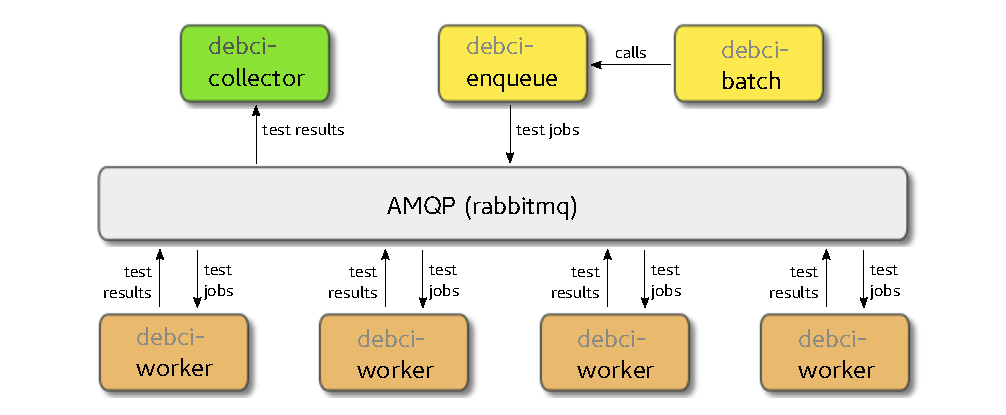
\includegraphics{./image201706/architecture.eps}
\caption{debci's architecture}
\end{figure}

Installation instructions:
\url{https://ci.debian.net/doc/file.INSTALL.html}

sudo apt install debci debci-collector debci-worker

It is also recommended to use \texttt{apt-cacher-ng} (not sure if just
installing is enough\ldots{}).

\subsubsection{Issues with the
installation.}\label{issues-with-the-installation.}

\textbf{\emph{Disclaimer: maybe everything works well and I did not
forget the instructions correctly? I did not have time to
triple-check.}}

Debci's documentation says: ``\emph{As usual, you will prompted for the
address of the AMQP server. If the rabbitmq-server is on the same host,
just leave it blank}''. In my case, I did not see a prompt. But since I
use a local server, there was no problem.

If there are problems with rabbitmq, it is useful to check at the web
interface. But it is not installed by default.

\begin{verbatim}
rabbitmq-plugins enable rabbitmq_management
\end{verbatim}

Then, visit \url{http://localhost:15672/} (login:guest,
password:guest0).

There is also a command-line tool to query the queues:
\texttt{rabbitmqadmin}.

\subsubsection{Other issues.}\label{other-issues.}

\url{https://bugs.debian.org/809652}: \emph{debci: setup sets stamps
even if setup failed}

This bugs prevents debci commands to try again when they should. For
example, this command fails for a good reason (lxc not installed).

\begin{verbatim}
$ sudo debci update-worker
Starting testbed setup: Tue May 30 21:17:47 JST 2017
E: lxc is not installed
Finished testbed setup: Tue May 30 21:17:47 JST 2017
\end{verbatim}

What happens if one configure lxc as needed and restarts the command ?

\begin{verbatim}
$ sudo debci update-worker
Starting testbed setup: Tue May 30 21:17:50 JST 2017
I: testbed already updated in the last 12h, no need to update
\end{verbatim}

It refuses to run for the next 12 hours !

Fortunately the solution is simple: there is a \texttt{-\/-force}
option.

The debci index generator was crashing and I could not debug the
problem, but I happened to have to reboot my laptop this week, and the
problem disappeared\ldots{} (Unfortunately, \texttt{systemd} did not
keep the logs of the previous boots\ldots{} how did I configure it so
wrong ?)

\subsubsection{Configuration}\label{configuration}

\texttt{lxc} is default, but I wanted to use \texttt{schroot}. Either I
had to pass \texttt{-\/-backend\ schroot} to all the commands, or I had
to add it to the configuration (same for \texttt{-\/-suite\ stretch}).i

The configuration files are in \texttt{/etc/debci/} and
\texttt{/debci/conf.d/}. By default, these directories are empty, with
no example files. But study of the
\href{https://github.com/terceiro/debci/blob/master/lib/environment.sh}{source
code} of debci indicates that the configuration files are sourced by the
shell to define environment variables. Further study of the debci code
suggested that the names of the variables can easily be guessed. So here
is my configuration.

\begin{verbatim}
$ cat /etc/debci/conf.d/local.conf 
debci_suite=stretch
debci_backend=schroot
\end{verbatim}

TODO: submit an example configuration file via the BTS\ldots{}

\subsubsection{Et c'est parti !}\label{et-cest-parti}

Let's test all R/Bioconductor packages in Squeeze.

\begin{verbatim}
apt-cache search r-bioc* | cut -f1 -d ' ' |  xargs debci enqueue
\end{verbatim}

And voil`a, \texttt{debci} did the rest.

\begin{verbatim}
$ ls /var/lib/debci/data/packages/stretch/amd64/r/ | more
r-bioc-affy
r-bioc-affyio
r-bioc-altcdfenvs
[ plus many more ...]
r-bioc-metagenomeseq
r-bioc-multtest
r-bioc-phyloseq
\end{verbatim}

\subsection{Conclusion}\label{conclusion}

I still have to dig in the results.

There seems to be some autogenerated HTML pages, but I still have to
figure out how to get nice diffs like on \texttt{ci.debian.net}. Example
file path:

\begin{verbatim}
file:///var/lib/debci/data/.html/packages/r/r-bioc-affy/stretch/amd64/index.html
\end{verbatim}

Final conclusion: I hope to use \emph{debci} more extensively during the
next release cycle to test potential backports.

%
% 冊子にするために、4の倍数にする必要がある。
% そのための調整
\dancersection{メモ}{}
\mbox{}\newpage
\mbox{}\newpage
\mbox{}\newpage


\vspace*{15cm}
\hrule
\vspace{2mm}
\includegraphics[width=2cm]{image200502/openlogo-nd.eps}
\noindent \Large \bf Debian 勉強会資料\\
\noindent \normalfont \debmtgyear{}年\debmtgmonth{}月\debmtgdate{}日 \hspace{5mm}  初版第1刷発行\\
\noindent \normalfont 東京エリア Debian 勉強会 (編集・印刷・発行)\\
\hrule

\end{document}
